\section{Enabling Silicon Photonic Technologies}
SiPh offer a variety of interesting devices that have the potential to be of tremendous power and performance benefit for HPC networks. Our proposal is based on three SiPh devices that--when combined--enable a powerful interconnect fabric: 1) Microring resonators (MRRs), 2) Arrayed Waveguide Grating Routers (AWGRs), and 3) color-blind switches (i.e. Micro-Electro Mechanical Systems (MEMS), Mach Zehnder Interferometers (MZI)). 

\subsection{Microring Resonators}
In order to understand the significance of MRRs to SiPh interconnects, it is useful to first discuss how data transmission is performed in an optical link. Figure~\ref{fig:olink} depicts an example optical link with all components needed to transmit data between a source-destination pair. 
\begin{figure}[!t]
	\centering
	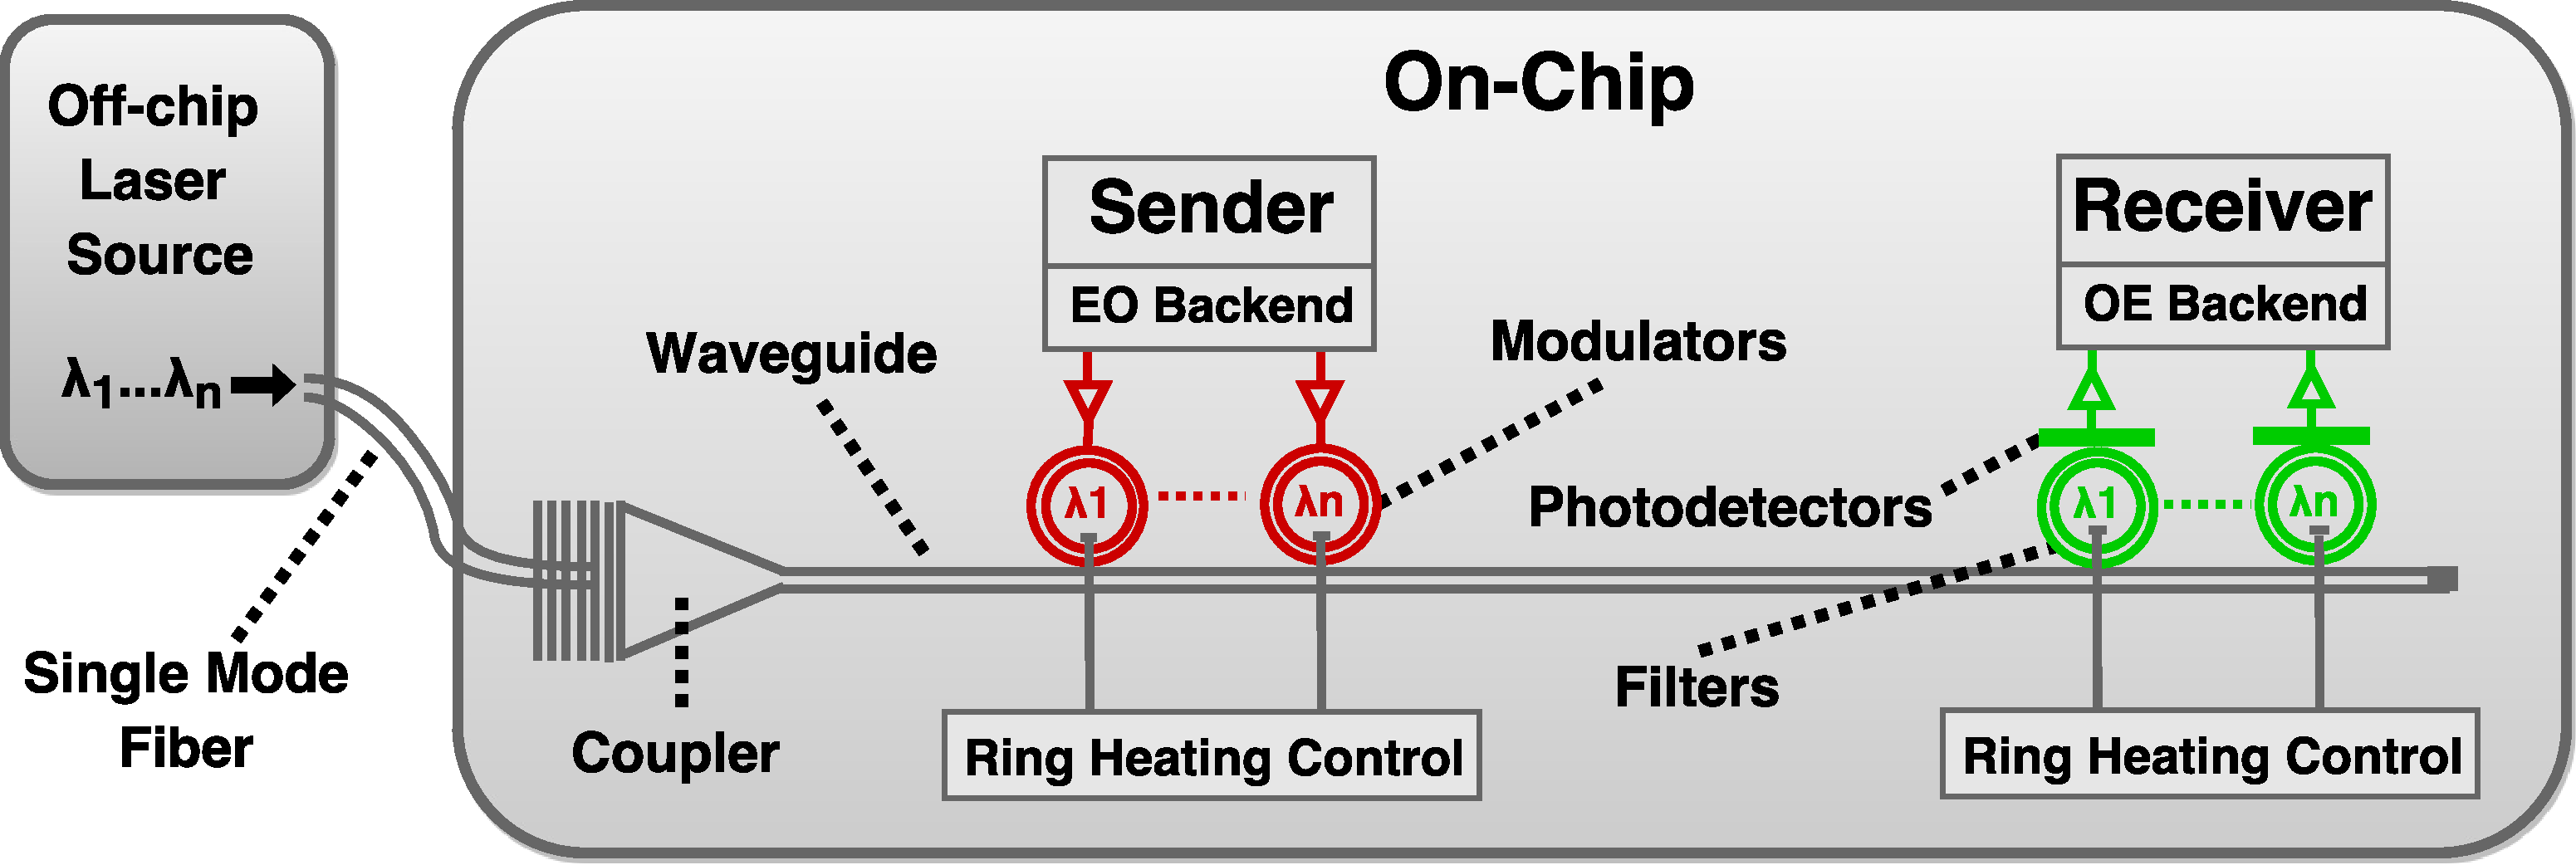
\includegraphics[width=\linewidth,clip]{latex/Figures/olink.pdf}
	\vspace{0.01cm}
	\caption[A Reference SiP Link]{A Reference SiP Link}
	\label{fig:olink} 
\end{figure}
Light generated from an off-chip laser is confined inside an optical fiber, which is then coupled into an on-chip waveguide. Modulators encode bits onto the optical medium (electrical-to-optical (EO) conversion), and filter-photodetector pairs extract the optical signal, performing optical-to-electrical (OE) conversion. Aside from steering particular wavelengths to a photodetector, MR filters are also deployed as switching devices since they allow to `drop' wavelengths from one waveguide to another, thereby allowing to implement wavelength-selective routing by strategically placing them between waveguides. \\
Optical signals can consist of multiple wavelengths ($\lambda _0 .. \lambda_n$) on which data can be transmitted in parallel--a technique commonly referred to as wavelength-division multiplexing (WDM). In order to exploit WDM, one modulator and MR filter per wavelength is needed at the sender and receiver, respectively. \\
MRs form the basis for both modulators and filters and are designed to respond to one particular wavelength channel (referred to as `resonance wavelength'); however, MRs are cyclic with the period--called the \textit{Free Spectral Range} (FSR)--meaning that an MR that drops wavelength $\lambda_i$ can also drop $\lambda_{i+ FSR*k}$ (with \textit{k} being an integer). A MR's resonance wavelength depends on device geometry/dimensions and the ambient temperature and variation thereof can cause the resonance wavelength to shift, effectively causing malfunctioning. While device mismatches during fabrication can be mitigated by MR trimming, protecting MRs from on-chip temperature variations requires integrated heaters ensuring thermo-optical control of each individual MR during operation. \\
Aside from ensuring correct behavior, integrated heaters can also be used deliberately to dynamically turn on/off MR filters. Changing the ambient temperature of a MR with heaters so that its resonance wavelength shifts beyond the free spectral range of all wavelengths on a link effectively allows to dynamically turn off (and on) a MR. Several previous studies leverage this approach to implement path setup and tear down functionality of circuit-switched optical networks based on wavelength-selective routing~\cite{bergman2014photonic}, which is also part of our proposed switching fabric. 

\subsection{Arrayed Waveguide Grating Router}\label{sec:awgr}
While all the wavelength routing functionality in an optical network could be implemented with MRs (as discussed above), networks solely relying on MRs to perform routing have several shortcomings, such as large power overheads for thermo-optical control of each MR, poor scalability (networks often require 1000s of MRs), excessive crosstalk, and the challenging task of finding a physical layout with low path losses~\cite{ramini2013contrasting}~\cite{boos2013proton}~\cite{hamedani2014qut}.\\
AWGRs overcome these challenges by providing scalable and low-loss wavelength routing on a passive platform that uses phase changes and constructive interference to enable an all-to-all $N \times N$ interconnection utilizing \textit{N} wavelengths and \textit{N} input and output waveguides~\cite{grani2017design}. Unlike MRs, AWGRs are less susceptible to temperature variations and do generally not require on-chip heating. 
In addition, recent advancements in CMOS-compatible SiN-based AWGRs enabled significantly reduced footprint ($<$1$mm^2$), low crosstalk ($<$-38dB) and loss ($<$2dB) values, giving AWGRs them a considerable edge to MR-based switching fabrics~\cite{shang2017low}. The physical layout of a fabricated SiN AWGR is illustrated in Figure~\ref{fig:awgrlayout}. \\
Figure \ref{fig:awgrmatrix} illustrates the wavelength distribution from the input to the output ports inside an $8\times 8$ AWGR. The wavelengths from each input port are evenly distributed to all output ports. 
\begin{figure*}[t!]
    \centering
        \begin{subfigure}[t]{0.18\linewidth}
        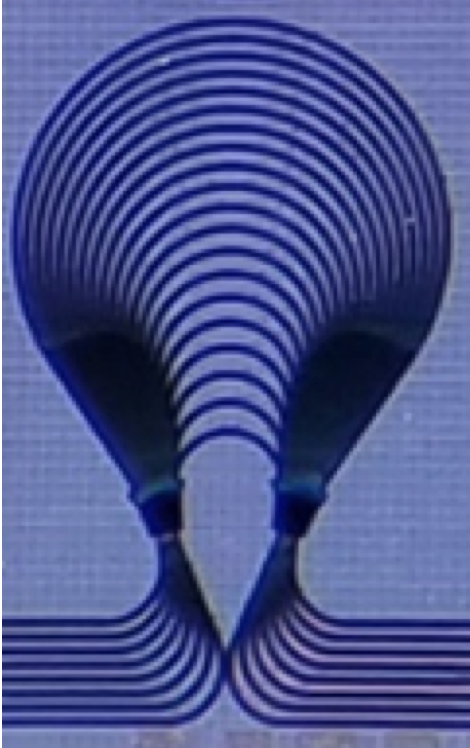
\includegraphics[width=\textwidth, clip]{Figures/awgrlayout.png}
        \caption{Physical Layout}
        		\label{fig:awgrlayout}
       \end{subfigure}
        \hspace{0.4cm}
        \begin{subfigure}[t]{0.46\linewidth}
        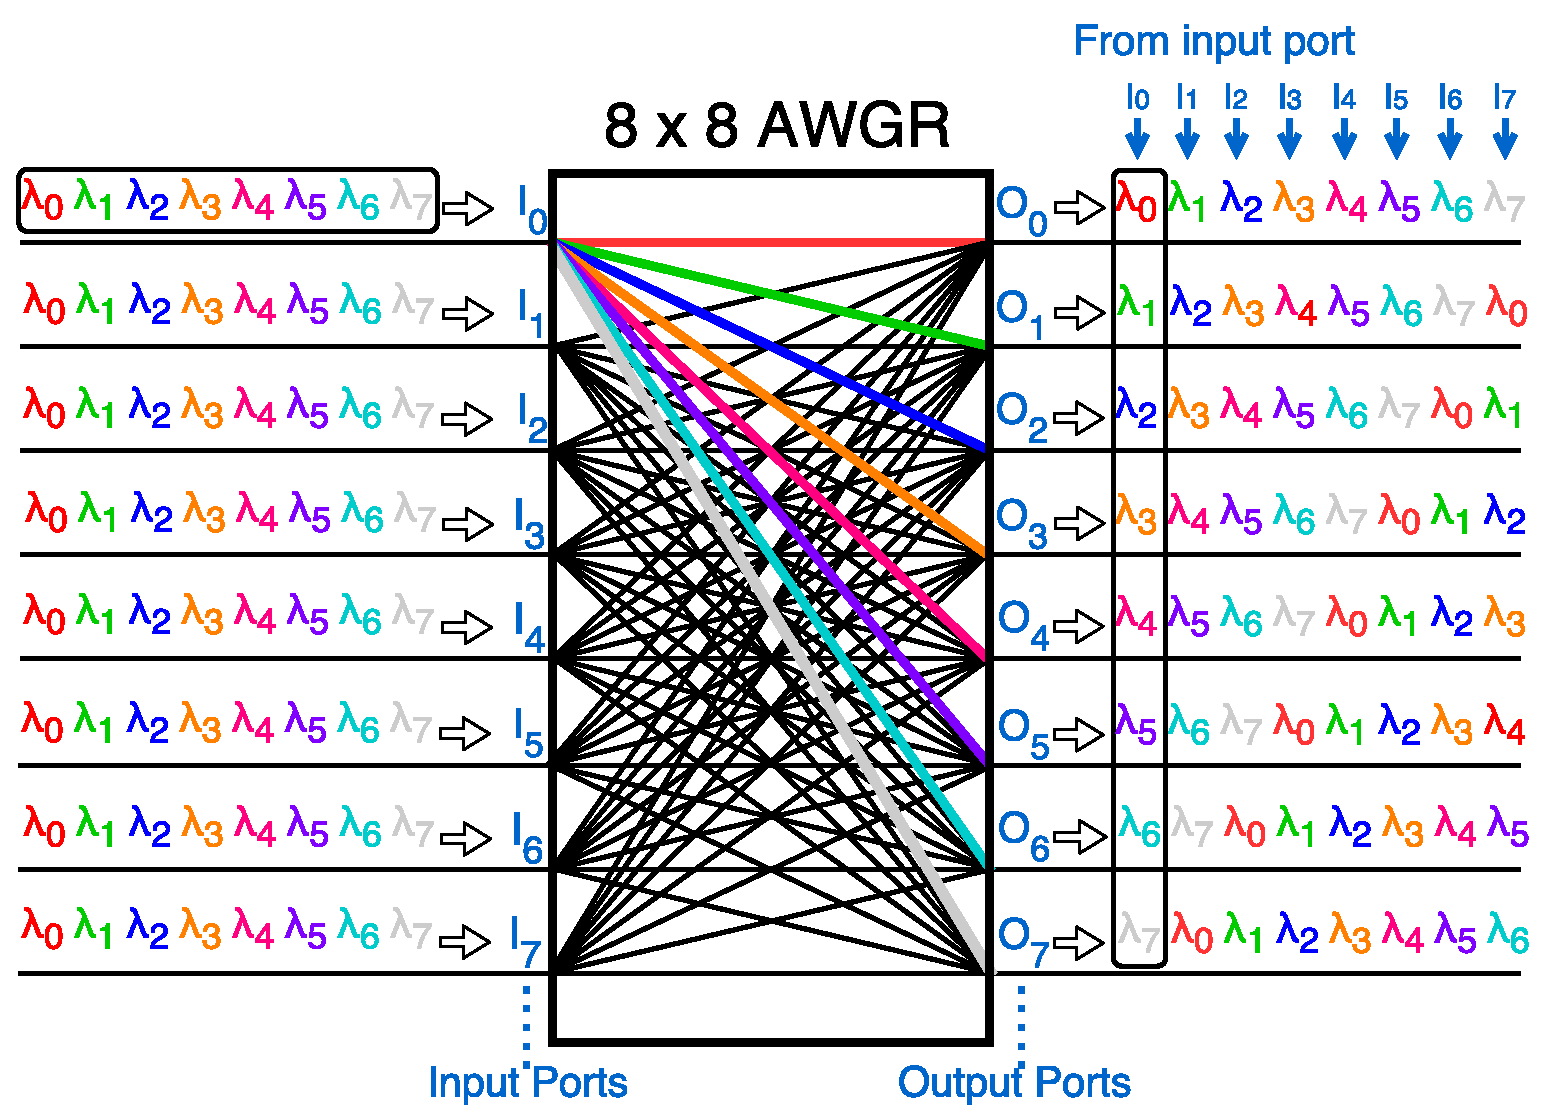
\includegraphics[width=\textwidth, clip]{Figures/awgr.pdf}
        \caption{Wavelength distribution inside an AWGR}
        		\label{fig:awgrmatrix}
    \end{subfigure}
        \hspace{0.4cm}
    \begin{subfigure}[t]{0.28\linewidth}
        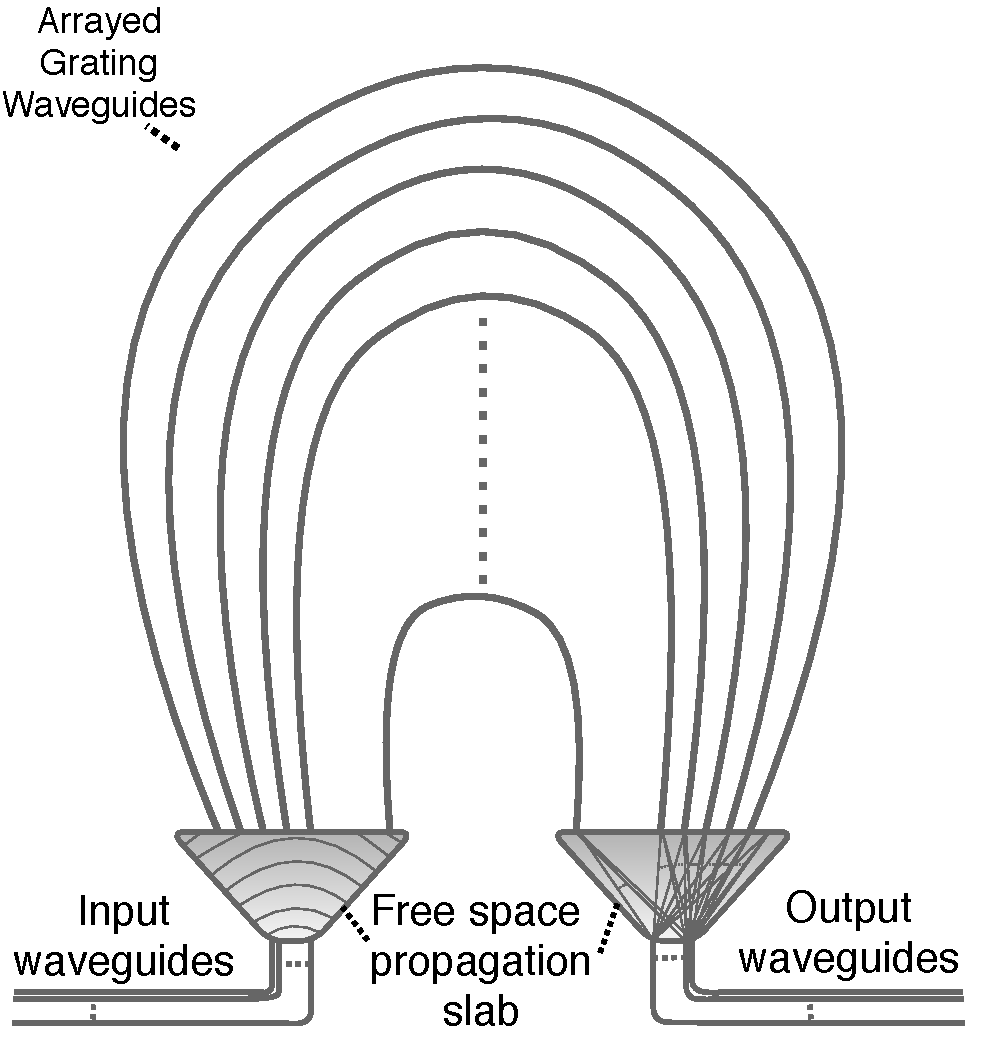
\includegraphics[width=\textwidth, clip]{Figures/awgrschematic.pdf}
        \caption{Schematic}
        		\label{fig:awgrcartoon}
    \end{subfigure}
    \caption[AWGR Structure and Switching Functionality]{Switching Functionality, Structure, and Layout of an 8$\times$8 AWGR}
\end{figure*}
This wavelength routing functionality is enabled by the constant phase change that each signal experiences when traversing the grating waveguides of an AWGR (see Figure~\ref{fig:awgrcartoon}) and is caused by the constant length increment of the grating waveguides. After traversing the grating waveguides, the wavelengths interfere constructively in the free space propagation region and get refocused at the output ports depending on their experienced phase shift.\\
It is important to note that, just like MRs, AWGRs are also cyclic with the period. Therefore, if input port \textit{i} can reach input port \textit{j} with wavelength $\lambda_{ij}$, \textit{i} can also reach \textit{j} with $\lambda_{ij + FSR*k}$ (with \textit{k} being an integer). This property has been exploited by previous studies to transmit multi-wavelength signals between source-destination pairs through an AWGR, referred to as \textit{bit-parallel AWGR}~\cite{grani2017bit}. 

\subsection{Color-blind switches}
*****TODO desribe and Compare MEMS/MZI/MRR crossbars *****\\
Problem: It's drawn in a figure 5 which doesn't appear until later ... TODO \\ 
\subsubsection{MEMS}
\subsubsection{MZI}
\subsubsection{MRR}
MEMS are color-blind SiP switches implementing a crossbar fabric with fast switching times, enabling rapid bandwidth reconfiguration. %Figure~\ref{fig:mems} (from~\cite{seok2016highly}) depicts an example $4 \times 4$ MEMS. 
%\begin{figure}[t!]
%        \includegraphics[width=\linewidth, clip]{Figures/mems.pdf}
%        \caption{From~\cite{seok2016highly}: (a) Depicts the structure of a MEMS switch with all its switching elements and input and output ports; (b) shows a close-up to a switching element, consisting of two layers of waveguides and a MEMS-Actuated Adiabatic Coupler; (c/d) illustrates the wavelength routing of the switching elements in OFF (c) and ON (d) state.}
  %      		\label{fig:mems}
%\end{figure}
Recently proposed MEMS switches proposed by researchers at UC Berkeley~\cite{seok2016highly} are particularly promising as they offer very low switching times (0.85$\mu$s), low on-chip insertion loss (8.5dB), low footprint ($1.9mm \times 1.9mm$ for a $16 \times 16$ MEMS), and, unlike MR-based fabrics, consume negligible on-chip power. \\
A MEMS has two layers of waveguides in crossbar mesh fabric and uses MEMS-actuated vertical adiabatic couplers as the switching elements (Figure~\ref{fig:mems}(b)). The optical operation bandwidth of adiabatic couplers ranges from 1400nm to 1700nm which is fully compatible with WDM networks. WDM signals entering an input port therefore either pass through to the `through ports' if all switching elements are in OFF state (Figure~ \ref{fig:mems}(c)) or are switched to one `drop port' if a switching element is in ON state.  \\
This structure allows each input port to reach every output port as long as the switching elements are (re)configured accordingly; however, MEMSs are color-blind switches and thus always switch \textit{all} wavelengths of a WDM to a certain output port. Variable bandwidth allocation is therefore not possible and each input can communicate only with one output at a time (simultaneous all-to-all connectivity like in AWGRs cannot be supported).  \\
In the following section, we show that MRs, AWGRs, and MEMS switches can, when co-integrated, be combined to form a powerful, highly-efficient, bandwidth-adaptive all-to-all interconnection fabric by exploiting the benefits of each device. 



